\subsection*{Channel Coding}
\underline{Produit scalaire de deux vecteur binaires $\overrightarrow{u}$ et $\overrightarrow{v}$}:

$\langle \overrightarrow{u},\overrightarrow{v}\rangle = u_1v_1\bigoplus u_2v_2\bigoplus\dots\bigoplus u_nv_n$.

\underline{Distance de Hamming}: nombre de positions où les bits de $\overrightarrow{u}$ et $\overrightarrow{v}$ diffèrent.

\underline{Distance minimale entre les mots code}: $d_{min}=\min \left\|\overrightarrow{u}\right\|$

\underline{Number of parity check-symbols}: $m=n-k$

\underline{Code length}: $n=2^m-1$

\underline{Number of information symbols}: $k=2^m-m-1$

\underline{Nombre d'erreurs}: $t$

\underline{Error correction capability condition}: $2t\leq d_{min}-1$

\underline{Rendement} $\eta=\sfrac{k}{n}$

\underline{Error detection capability}: $d_{min}-1$

\underline{Error correction capability condition}: $2t\leq d_{min}-1$

\columnbreak

\textbf{Hamming code}

\begin{figure}[H]
    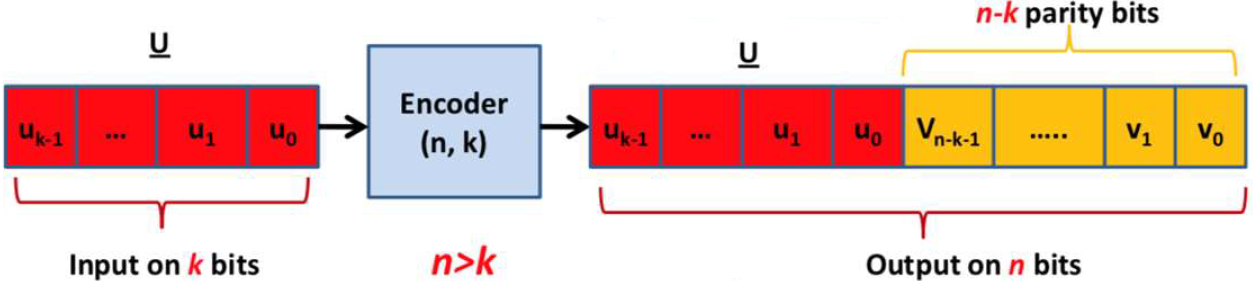
\includegraphics[width=\linewidth]{images/linear_block_codes.png}
\end{figure}
Si le mot à coder est $\overrightarrow{x}$ :

\underline{Encoder}: $G_s = (I_{k\times k}|P_{k\times n-k})$.

\underline{Decoder}: $H_s = (P_{n-k\times k}^T|I_{n-k\times n-k})$.

\underline{Code }: $\overrightarrow{y} = \overrightarrow{x}G_s$.

\underline{Erreur pendant la transmission}: $\overrightarrow{y_e}=\overrightarrow{y}+\overrightarrow{e}$.

\underline{Syndrome}: $\overrightarrow{s}= \overrightarrow{y}H_s^T+\overrightarrow{e}H_s^T$.

Pour mettre une matrice sous forme systématique il faut faire une combinaison linéaire des lignes ou colonnes.

Matrice de contrôle pour un code de Hamming (7,4) :

\setlength{\abovedisplayskip}{-2pt}
\setlength{\belowdisplayskip}{-2pt}
\begin{wrapfigure}{l}{5cm}
    \begin{equation*}
        H = \begin{pmatrix}
            0 & 0 & 0 & 1 & 1 & 1 & 1 \\
            0 & 1 & 1 & 0 & 0 & 1 & 1 \\
            1 & 0 & 1 & 0 & 1 & 0 & 1
        \end{pmatrix}
    \end{equation*}
\end{wrapfigure}
Dans ce cas $H\neq H_s$ car elle n'est pas canonique symétrique.
Si $\overrightarrow{s} = 0$ alors il n'y a pas d'erreur, sinon il y a une erreur. La position de
l'erreur est donnée par le syndrome. Il faut donc soustraire le syndrome à $\overrightarrow{y}$
pour trouver le mot d'origine.

Table avec quelques codes de Hamming et rendement associé:

\begin{tabular}{|ccccccc|}
    \hline
    $n - k$ & 2     & 3     & 4     & 5     & 6     & 7     \\
    \hline
    $n$     & 3     & 7     & 15    & 31    & 63    & 127   \\
    \hline
    $k$     & 1     & 4     & 11    & 26    & 57    & 120   \\
    \hline
    $\eta$  & 0.333 & 0.571 & 0.733 & 0.839 & 0.905 & 0.945 \\
    \hline
\end{tabular}

\textbf{Cyclic code}

\underline{Un code linéaire} (n, k) est dit cyclique si tout décalage cyclique d'un mot code est encore un mot code.

\setlength{\intextsep}{-5pt}
\begin{wrapfigure}{l}{0.2\textwidth}
    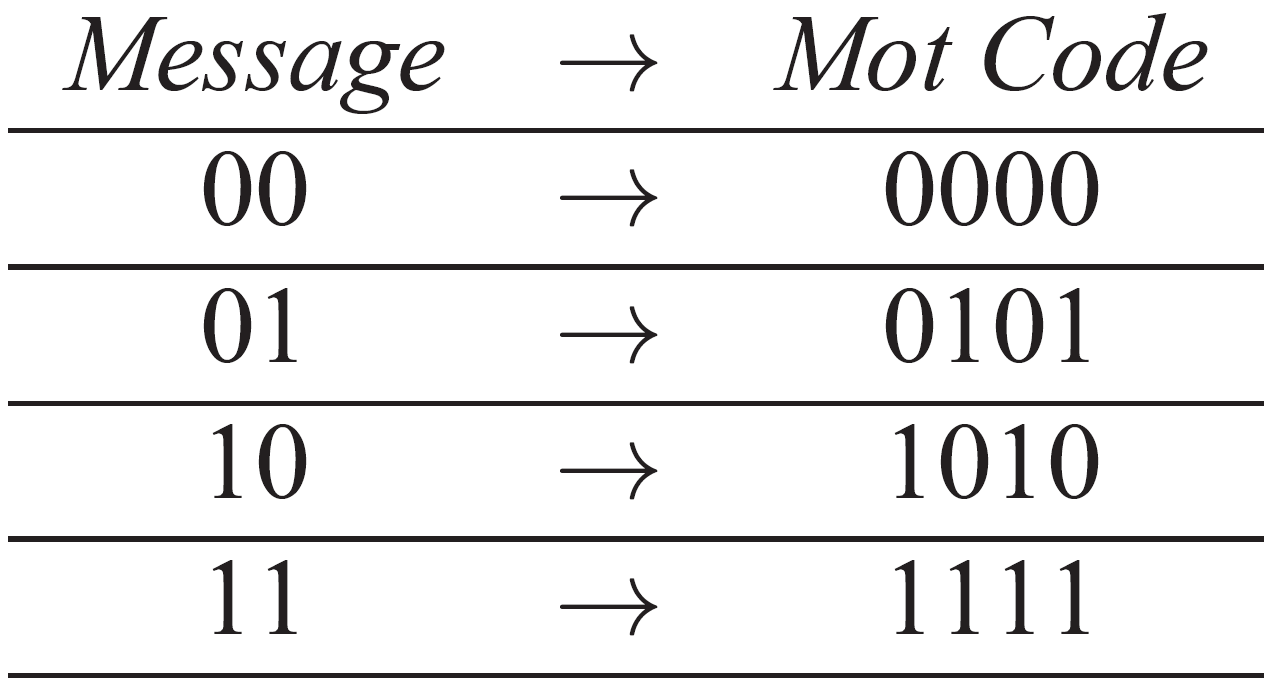
\includegraphics[width=\linewidth]{images/code_cyclique.png}
\end{wrapfigure}
\underline{Propriété 1:}

Le générateur d'un code cyclique est le code polynomial non nul de
degré minimal. Pour le cas dans le tableau: $0101$ s'écrit donc $0X^3 + 1X^2 + 0X + 1 =X^2+1$
qui est bien de degré $4-2 = 2$

\underline{Propriété 2:}

Le code polynomial non nul de degré minimal d'un code cyclique
(n, k) divise le polynôme $1 + X^n$ : $(1 + X^2)(1 + X^2) = 1 + 2X^2 + X^4 = 1 + X^4 + (1 + 1)X^2 = 1 + X^4$
(addition binaire donc $1+1=0$)

\columnbreak

\underline{Propriété 3:}

Afin d'engendrer le code on multiplie les polynômes correspondant
aux messages d'information par le polynôme générateur.

\setlength{\intextsep}{-2pt}
\begin{figure}[H]
    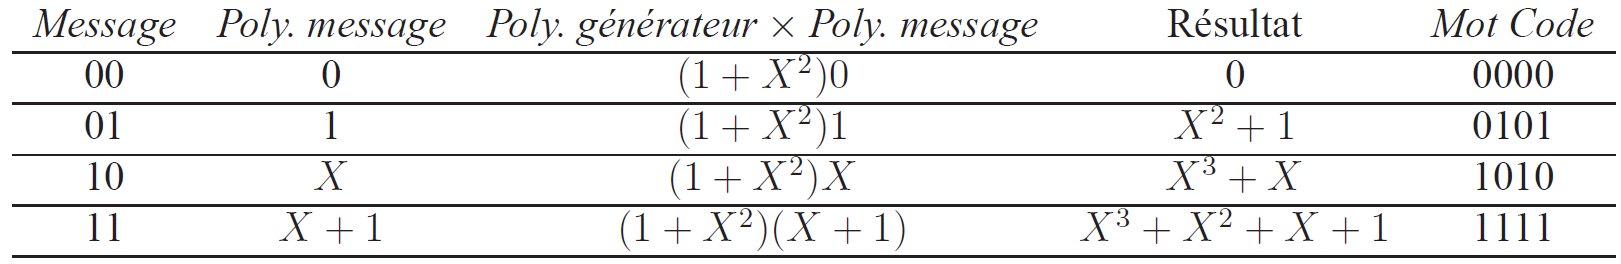
\includegraphics[width=\linewidth]{images/generer_code_cyclique.png}
\end{figure}

\underline{Propriété 4:}

Les k décalages cycliques du mot code correspondant au polynôme
non nul de degré minimal forment une base du code :
$0000 = 0 \times 1010 = 0 \times 0101$, $1010 = 1 \times 1010$, $0101 = 1 \times 0101$ et
$1111 = 1 \times 0101 + 1 \times 1010$

\textbf{Encodage systématique:} (n, k)

$G_s = (I_{k\times k}|P_{k\times n-k})$.
L'encodage systématique permet de retrouver le message d'origine en ne prenant que les
$k$ premiers bits du mot code, les $n-k$ derniers bits sont les bits de parité.

\underline{Multiplier le message:} $i(X)\rightarrow X^{n-k}i(X)$.

\underline{Diviser par le polynôme générateur}: $X^{n-k}i(X)=a(X)g(X)+r(X)$

\underline{Ajouter le reste à la fin du message} compte tenu de l'addition binaire:

$X^{n-k}i(X)+r(X)=a(X)g(X)$

\underline{Exemple}:

Trouver pour un code cyclique (7, 4) l’encodage systématique de $1010$.

Trouver le générateur: $1+X^7=(1+X)(1+X+X^3)(1+X^2+X^3)$, on prend $g(X)=1+X+X^3$.

Calculer: $X^{n-k}i(X)=X^3(X^3+X)=X^6+X^4$.

\setlength{\abovedisplayskip}{-2pt}
\setlength{\belowdisplayskip}{-2pt}
\begin{wrapfigure}{l}{6cm}
    \[
        \begin{array}{r|r}
            X^6 + X^4\phantom{{}+6} & X^3 + X + 1 \\ \cline{2-2}
            + X^6 + X^4 +X^3        & X^3 + 1     \\ \cline{1-1} \\[\dimexpr-\normalbaselineskip+\jot]
            X^3\phantom{{}+6}                     \\
            +X^3 + X + 1                          \\ \cline{1-1} \\[\dimexpr-\normalbaselineskip+\jot]
            X + 1
        \end{array}
    \]
\end{wrapfigure}
Diviser par $g(X)$: $X^6+X^4=(X^3 + X + 1)(X^3 + 1)+X+1$

Ajouter le reste au calcul: $X^6+X^4+X+1\rightarrow 1010011$

Schéma équivalent au circuit de division $\frac{u(X)}{g(X)}$
\vspace*{0.5cm}
\begin{figure}[H]
    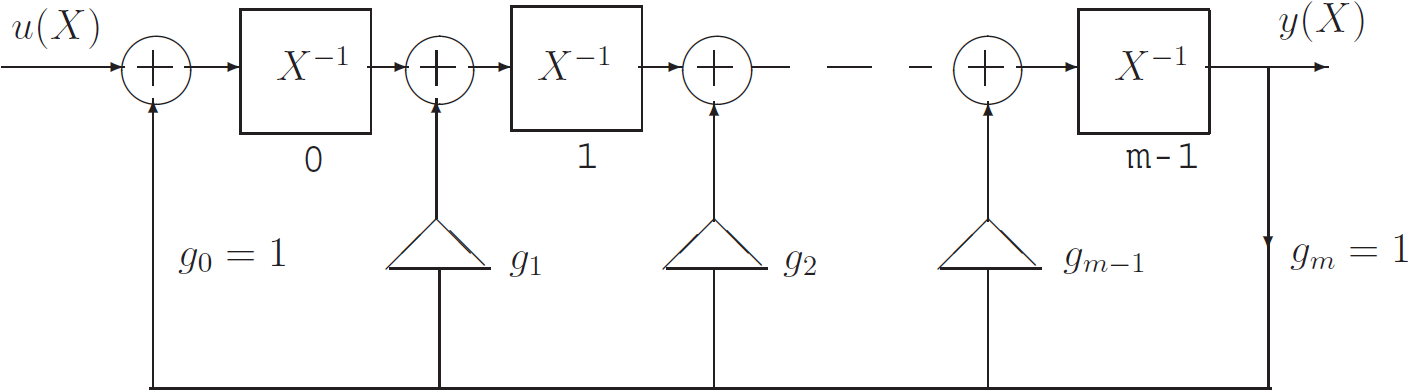
\includegraphics[width=\linewidth]{images/schema_division.png}
\end{figure}

\columnbreak

\underline{Décodage:}

On divise le block reçu par $g(x)$, si le reste est nulle le
résultat est juste autrement il est faux. Le syndrome est
le reste de la division par $g(x)$.

On calcule un code à partir du message reçu puis on
compare ce code avec celui qui est reçu. Ceci ne marche
que pour les codes systématiques.

\textbf{BCH code:}

Les codes BCH sont construits pour corriger t erreurs. Pour
tout couple d'entiers positifs $m$ $(m \geq 3)$ et $t$ $(t < 2m-1)$ on peut
montrer qu'il existe un code binaire BCH avec les
paramètres suivants :

\underline{Number of parity check-symbols}: $n-k\leq mt$.

J'ai rien compris ça à l'air trop compliqué.

\textbf{Convolutional code:}

Les codeurs convolutifs ont une mémoire qui influe sur les $n$ bits de sortie à partir des $k$
bits d'entrée et des $m$ états internes.

\underline{Taux de codage}: $R=\frac{1}{n}$

\underline{Code state}: le contenu de la mémoire, il y a $2^{mk}$ états différents.

\underline{Exemple de diagramme}: $n=2$, $k=1$, $m=3$ (2,1,3)

\begin{figure}[H]
    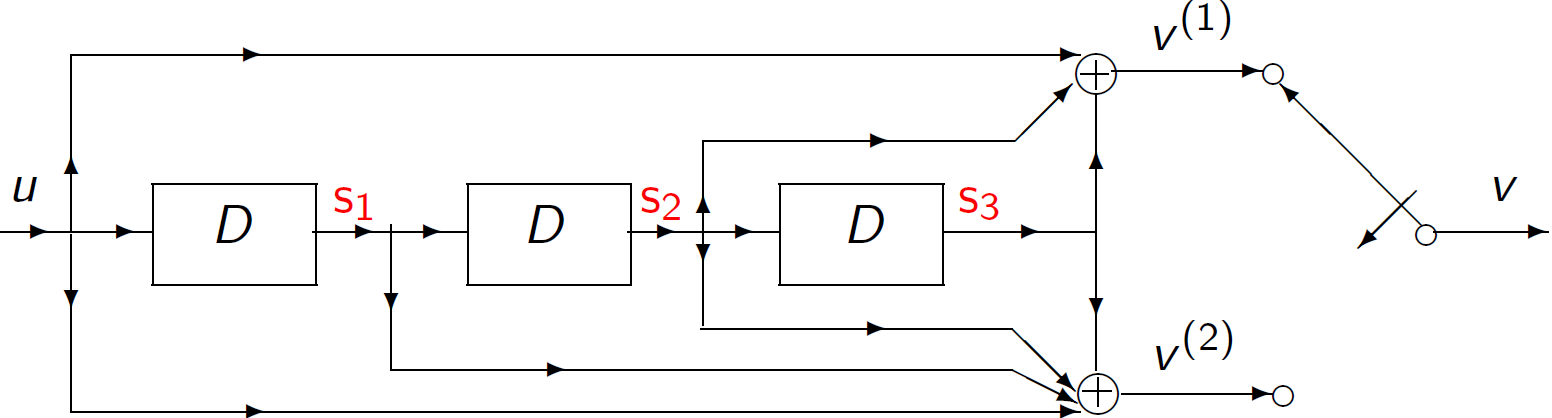
\includegraphics[width=\linewidth]{images/conv_coding_diagramme.png}
\end{figure}

Pour chaque état on peut trouver on trouve la dépendance temporelle :
$s_1=u(n-1)$,

$s_2=s_1(n-1)$,

$s_3=s_2(n-1)$

Pour chaque output écrire leur dépendance :

$v^{(1)}=u(n)+s_2(n)+s_3(n)$,

$v^{(2)}=u(n)+s_1(n)+s_2(n)+s_3(n)$

En transformée de Z cela donne:

$V^{(1)}(z)=(1+z^{-2}+z^{-3})U(z)$,

$V^{(2)}(z)=(1+z^{-1}+z^{-2}+z^{-3})U(z)$

Les polynômes générateurs sont:

$g^{(1)}=(1,0,1,1)$,

$g^{(2)}=(1,1,1,1)$.

$V^{(1)}$ est donc la convolution entre $u(n)$ et $g^{(1)}$.

\columnbreak
\underline{Exemple complet}:
\begin{figure}[H]
    \begin{minipage}{0.255\textwidth}
        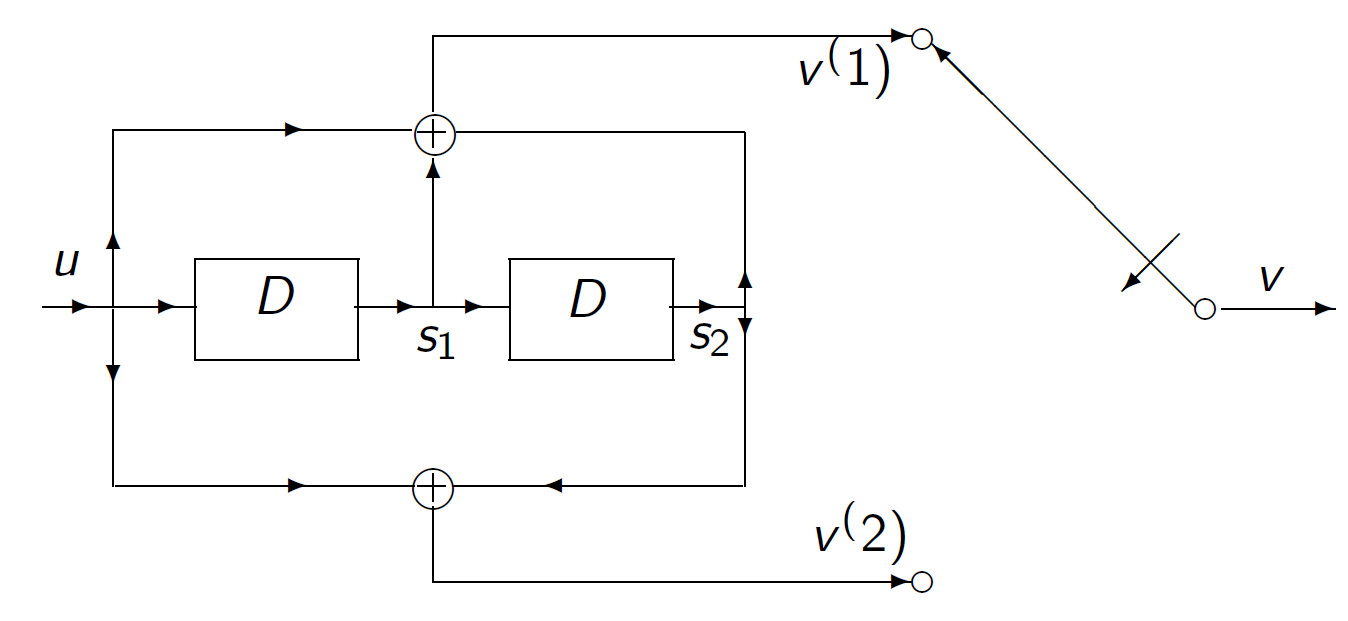
\includegraphics[width=\linewidth]{images/conv_coding_diagramme_2.png}
    \end{minipage}%
    \begin{minipage}{0.255\textwidth}
        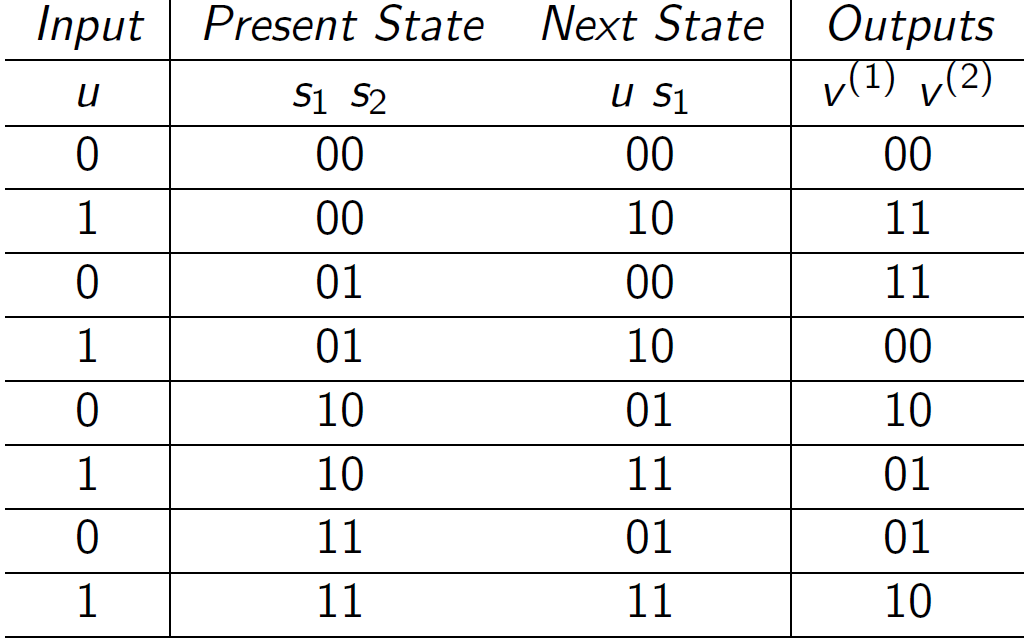
\includegraphics[width=\linewidth]{images/conv_coding_table_2.png}
    \end{minipage}
\end{figure}
L'\underline{encoder state diagram} (droite): représente les états du codeur et les transitions entre
les états.

En rouge \textcolor{red}{les états}, en bleu \textcolor{blue}{les inputs} (nouvelles
valeurs de $u(n)$) et en vert \textcolor{green}{les outputs} (valeurs de $v(n)$).

De Cela on peut construire le \underline{diagramme de treillis} (gauche) qui représente les chemins
possibles dans le codeur.
\begin{figure}[H]
    \begin{minipage}{0.15\textwidth}
        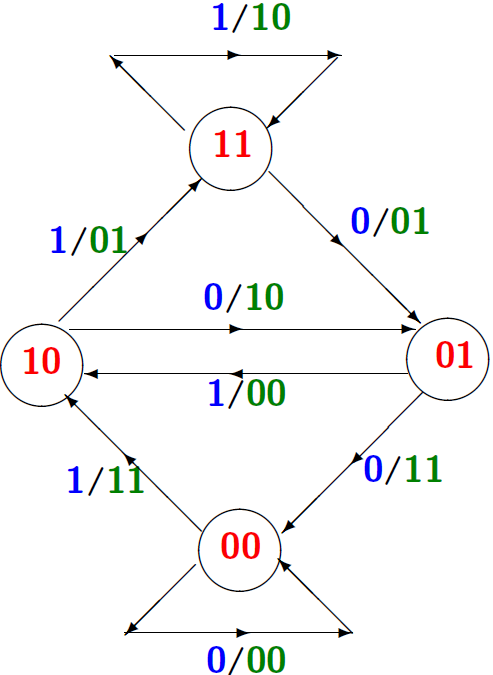
\includegraphics[width=\linewidth]{images/conv_coding_encoder_state_diagram_2.png}
    \end{minipage}%
    \begin{minipage}{0.35\textwidth}
        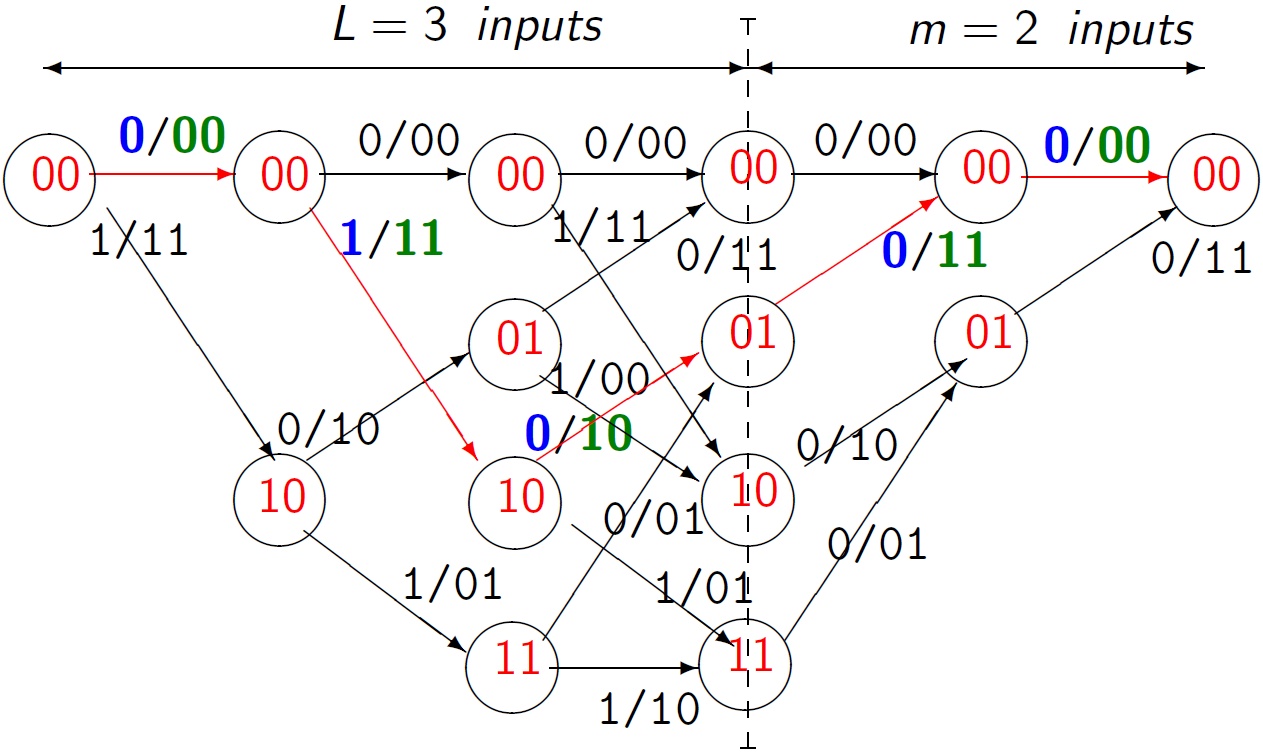
\includegraphics[width=\linewidth]{images/conv_coding_treillis_diagram_2.png}
    \end{minipage}
\end{figure}
Ce diagramme de treillis représente la réponse à une entrée \textcolor{blue}{$u(n)=010$} qui donne en sortie
\textcolor{green}{$v(n)=0011101100$}.

Le décodeur d'un code convolutif cherche le chemin dans le treillis qui correspond le
mieux aux données reçues (l'observation) on utilise \underline{l'algorithme de Viterbi} pour cela.
Le best fit peut se calculer de deux manières différentes:

Par la distance de Hamming entre les bits reçus et attendus.

Par la distance euclidienne au carré entre les valeurs reçues et attendues.
\begin{figure}[H]
    \begin{minipage}{0.24\textwidth}
        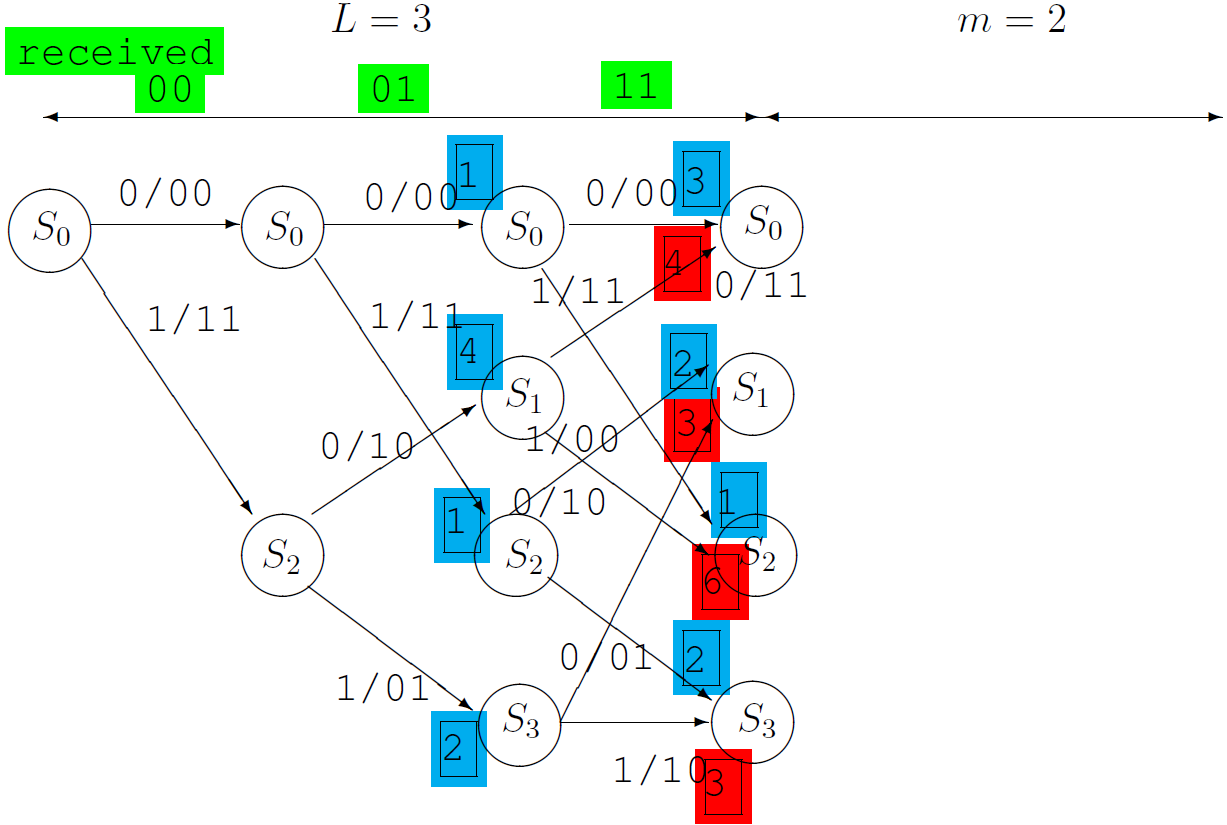
\includegraphics[width=\linewidth]{images/conv_coding_viterbi_1.png}
    \end{minipage}
    \begin{minipage}{0.24\textwidth}
        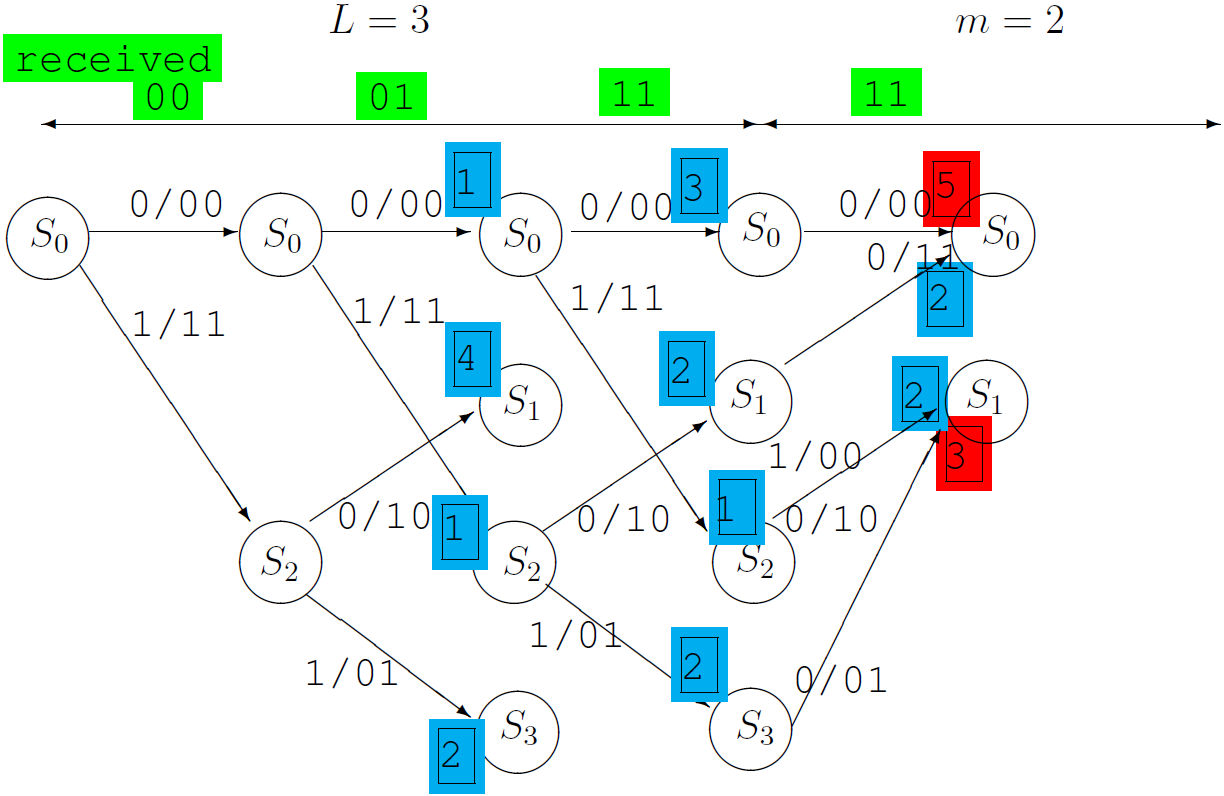
\includegraphics[width=\linewidth]{images/conv_coding_viterbi_2.png}
    \end{minipage}
\end{figure}
\needspace{5\baselineskip}
\begin{wrapfigure}{l}{0.24\textwidth}
    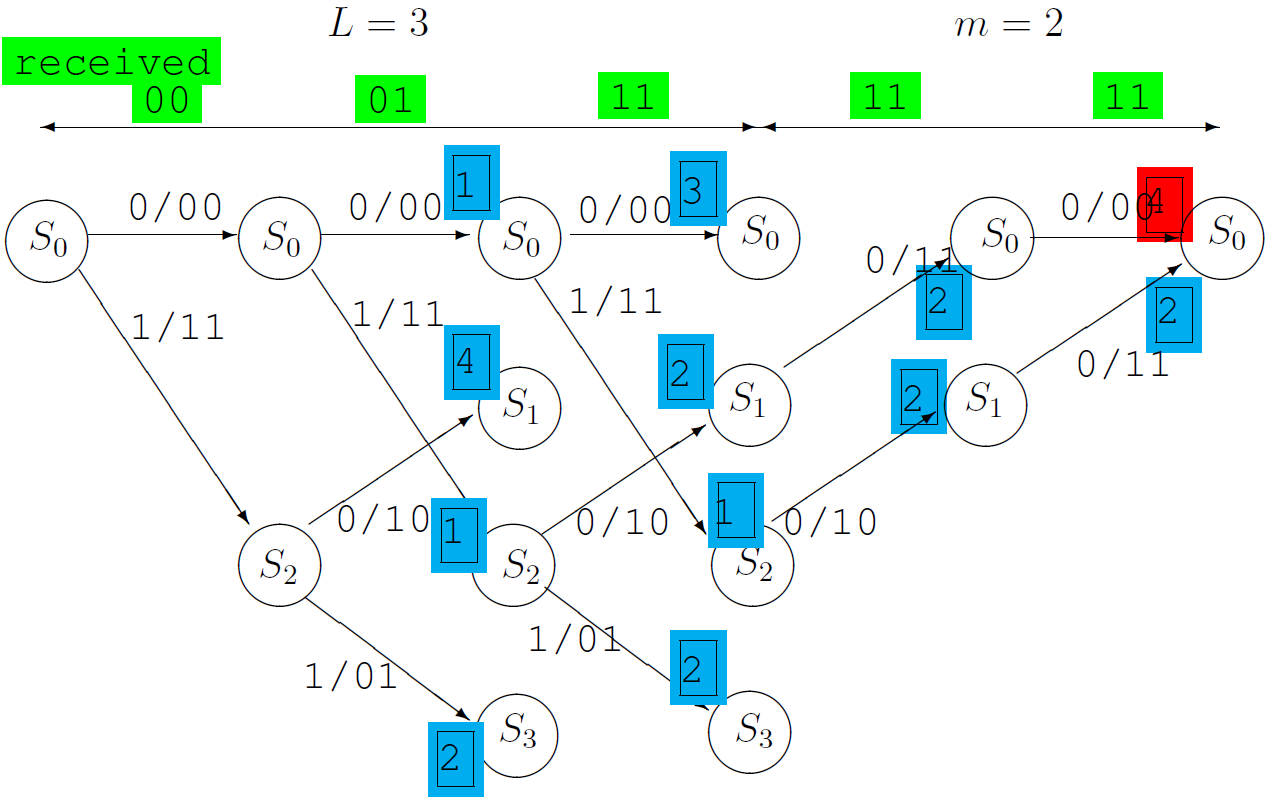
\includegraphics[width=0.24\textwidth]{images/conv_coding_viterbi_3.png}
\end{wrapfigure}
Le message transmis est : $00 01 11 11 11$ en utilisant la distance de Hamming comme metric pour
le best fit. Dans ce cas on trouve un chemin avec un distance de Hamming de 2. Le message corrigé est
$00 00 11 10 11$ la séquence d'entrée détectée est $001$.\\






